%---------------------%
\subsection{High-level components and their interaction}
In the following section is provided an high view of the architecture of the system, that is structured following the three logic layer:\\

\begin{figure}[H]
    \begin{center}
    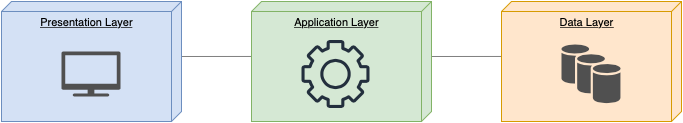
\includegraphics[width=1.2\textwidth]{images/System architecture.png}
    \caption{three layer architecture}
    \label{fig:system architecture}
    \end{center}
\end{figure}

\begin{itemize}
    \item \textbf{Presentation Layer (P)}: The presentation tier is the user interface and communication layer of the application, where the end user interacts with the application. Its main purpose is to display information to and collect information from the user. This top-level tier can run on a web browser, as desktop application, or a graphical user interface (GUI), for example. \\ \\Web presentation tiers are usually developed using HTML, CSS and JavaScript. Desktop applications can be written in a variety of languages depending on the platform.
    \item \textbf{Business Logic or Application Layer(L)}: The application tier is the heart of the application. In this tier, information collected in the presentation tier is processed - sometimes against other information in the data tier - using business logic, a specific set of business rules. The application tier can also add, delete or modify data in the data tier.\\ \\The application tier is typically developed using Python, Java, Perl, PHP or Ruby, and communicates with the data tier using API calls. 
    \item \textbf{Data Layer (D)}: The data tier, sometimes called database tier, data access tier or back-end, is where the information processed by the application is stored and managed. This can be a relational database management system such as PostgreSQL, MySQL, MariaDB, Oracle, DB2, Informix or Microsoft SQL Server, or in a NoSQL Database server such as Cassandra, CouchDB or MongoDB. 
\end{itemize}

In this case the system is a distributed application that follows the client-server paradigm: it is a two-tier architecture, consisting of a presentation and a data tier. the business logic lives in the data tier only.
In a two-tier application, all communication goes through the application tier. The presentation tier and the data tier cannot communicate directly with one another. 

Client and server are being allocated into different physical machines and their communication takes place via other components and interfaces, located in the middle of the structure and composed by hardware and software modules. 
The client is a Web Application, with is by definition a thin client, because of its total dependency from the server; so it only contains the presentation layer.

\begin{figure}[H]
    \begin{center}
    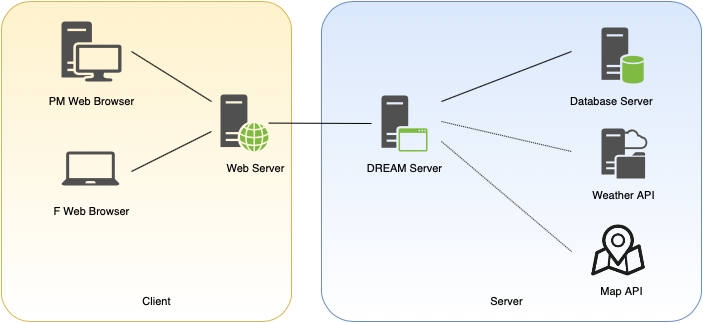
\includegraphics[width=1.2\textwidth]{images/System diagram.png}
    \caption{Dream system diagram.}
    \label{fig:system diagram}
    \end{center}
\end{figure}

\begin{itemize}
    \item \textbf{Server side:}
        \begin{itemize}
            \item \underline{ApplicationServer (DREAM Server)}: it is the central point of the system. Is a server whit all the application logic, that communicates with the other servers. 
            \item \underline{Database Server}: this is the server where all the application data are stored.
            \item \underline{Weather API}: external API used to retrieve data about weather in the territory. This information will be used to fill each farm page.
            \item \underline{Map API}: external API used to retrieve data about the territory.
        \end{itemize}
    \item \textbf{Client side:}
        \begin{itemize}
            \item \underline{Policy Maker Web Browser}: browser used by the policy maker from their work desk to access to the system
            \item \underline{Farmer Web Browser}: browser used by the farmer to access to the system
        \end{itemize}
\end{itemize}


%---------------------%
\subsection{Component view}

In this section is provided a description of the components and interfaces of the system, how they are organised internally and how they comunicate with each other.

\begin{figure}[H]
    \begin{center}
    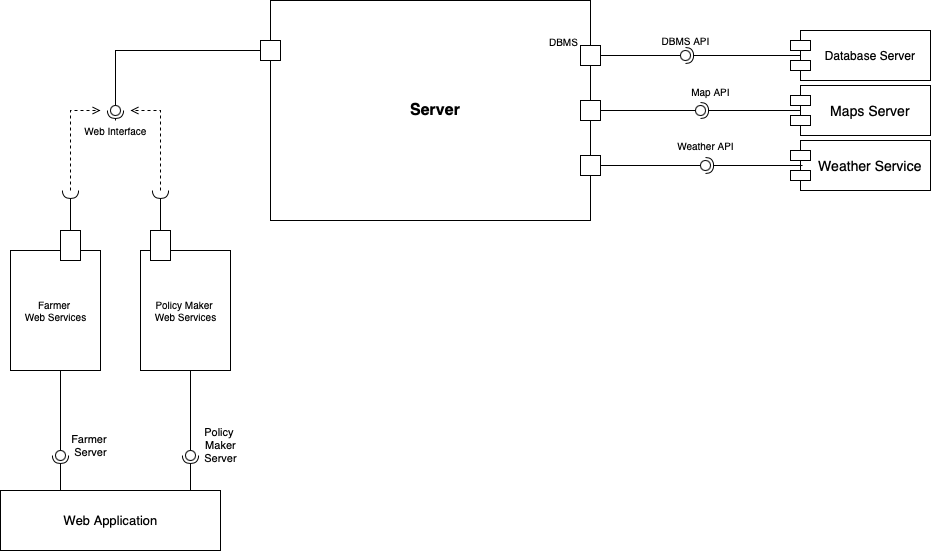
\includegraphics[width=1.2\textwidth]{images/Component1.png}
    \caption{Component view.}
    \label{fig:component view}
    \end{center}
\end{figure}

\begin{figure}[H]
    \begin{center}
    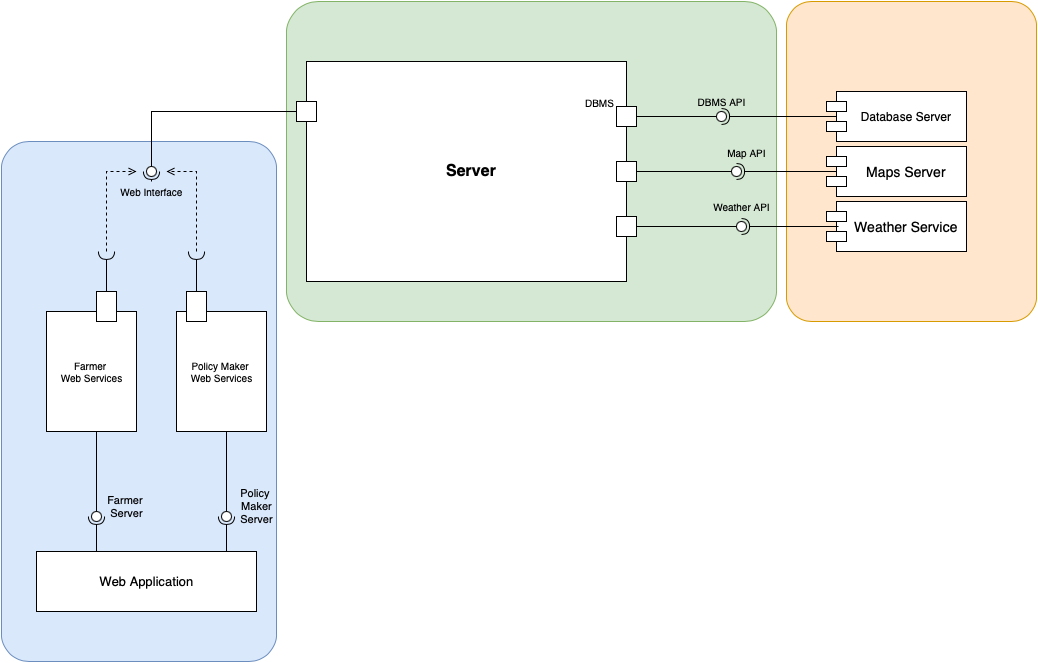
\includegraphics[width=1.2\textwidth]{images/Component2.png}
    \caption{Component view.}
    \label{fig:component view2}
    \end{center}
\end{figure}

%---------------------%
\subsection{Deployment view}

%---------------------%
\subsection{Runtime view}

In this section the focus is on the specific (dynamic) interaction between the components of the system; in other world the behaviour of the system at runtime.
The functionality offered by the component are the same as the ones in the RASD, but this time the focus is on how the internal components provides it.
(MAKE SURE THAT THE OPERATION AND COMPONENT ARE ALL DEFINED IN THE COMPONENT DIAG/VIEW, in particular the interfaces that receives the msg)

\begin{enumerate}
    \item farmer registration
    \item f/pm login
    \item f send msg on forum
    \item f submit production data
    \item f/pm find farm on the map
    \item f/pm visualize farm info (page)
    \item submit notification (f: help, advice | pm: solution)
    \item f/pm visualize notificationpm ipdate the map (evaluation)
\end{enumerate}

%---------------------%
\subsection{Component interfaces}

%---------------------%
\subsection{Architectural styles and patterns}

%---------------------%
\subsection{Other design decisions}

